% Baccalauréat malgache, série C, 2012 : corrigé.
\TCDBacAttribution{C}{2012}
\providecommand{\cm}{~\mathrm{cm}}
\providecommand{\Plan}{(\mathscr{P})}
\providecommand{\dx}{~\mathrm{d}x}
\providecommand{\dt}{\mathrm{d}t}
\providecommand{\Ouv}{(O;\vec{u},\vec{v})}
\providecommand{\mes}[2]{\mathrm{mes}\left( \widehat{ \overrightarrow{#1} ; \overrightarrow{#2} } \right)}
\providecommand{\D}{(\mathscr{D})}
\providecommand{\Courbe}{(\mathscr{C})}
\providecommand{\Courben}{(\mathscr{C}_n)}
\providecommand{\CourbeU}{(\mathscr{C}_1)}
\providecommand{\CourbeD}{(\mathscr{C}_2)}
\providecommand{\bary}[1]{\mathrm{bar}\left\lbrace #1 \right\rbrace}
\providecommand{\congru}[3]{#1 \equiv #2 \quad \left[ \mathrm{mod}~#3\right]}
\providecommand{\Angl}[2]{\left( \widehat{ \overrightarrow{#1} , \overrightarrow{#2} } \right)}
%
%%%%%%%%%%%%%%%%%%%%%%%%%%%%%%%%%%%%%%%%%%%%%%%%%%%%%%%%%%%%%%%%%%%%%%%%%%%%%%%%%%%%%%%%%%%%%%%%%%%%%%%%%%%%%%%%%%%%%%%%%%%%%%%%
\noindent \underline{\textsc{\textbf{Exercice}}} (4 points)
\begin{enumerate}
	\item Soit $(x_0 ; y_0)$ une solution de (E) (l'énoncé dit « la solution » : il faut lire « une solution »).
	\begin{enumerate}
		\item \vln{$4x_0 \equiv 2 \pmod 7$ :}
			$11x_0 = 9 + 7y_0$, donc $11x_0 \equiv 9 \pmod 7$. Comme $11 \equiv 4$ et $9 \equiv 2 \pmod 7$ :
			\par\noindent\ansbox{$4x_0 \equiv 2 \pmod 7$.}
		\item \vln{Solution particulière :}
			En multipliant par $2$ (car $4 \times 2 = 8 \equiv 1 \pmod 7$) : $x_0 \equiv 4 \pmod 7$.
			Pour $x_0 = 4$ : $7y_0 = 44 - 9 = 35$, $y_0 = 5$.
			\par\noindent\ansbox{$(4 \, ; 5)$ est une solution particulière de (E).}
		\item \vln{Résolution :}
			$11x - 7y = 9 = 11 \times 4 - 7 \times 5 \iff 11(x - 4) = 7(y - 5)$.
			$7$ divise $11(x-4)$ et $\pgcd{7}{11} = 1$, donc $7$ divise $x - 4$ : $x = 4 + 7k$, puis $y - 5 = 11k$. Réciproquement ces couples conviennent.
			\par\noindent\ansbox{$S = \{(4 + 7k \, ; 5 + 11k) \mid k \in \mathbb{Z}\}$.}
		\item \vln{Couple $(a,b)$ avec $11a - 7b = \pgcd{a}{b}$ :}
			Posons $d = \pgcd{a}{b}$, $a = da'$, $b = db'$ avec $\pgcd{a'}{b'} = 1$. L'égalité devient $11a' - 7b' = 1$.
			Or $11 \times 2 - 7 \times 3 = 1$ : $(a',b') = (2,3)$ convient (et $\pgcd{2}{3} = 1$).
			\par\noindent\ansbox{Par exemple $(a,b) = (2,3)$ : $22 - 21 = 1 = \pgcd{2}{3}$.}
			Plus généralement $(2d \, ; 3d)$ convient pour tout $d \geq 1$, par exemple $(18 ; 27)$ : $198 - 189 = 9 = \pgcd{18}{27}$.
	\end{enumerate}
	\item \textit{L'énoncé ne décrit que cinq faces (une face 2, deux faces 3, deux faces 4) pour un dé à six faces ; on adopte la lecture la plus probable :
		une face marquée 2, deux faces marquées 3 et trois faces marquées 4.}
		Ainsi $P(2) = \frac{1}{6}$, $P(3) = \frac{1}{3}$, $P(4) = \frac{1}{2}$, et les trois lancers sont indépendants.
	\begin{description}
		\item[$A$ :] \vln{Chiffres premiers seulement :}
			$2$ et $3$ sont premiers, $4$ ne l'est pas : chaque chiffre doit être $2$ ou $3$, de probabilité $\frac{1}{6} + \frac{1}{3} = \frac{1}{2}$.
			$P(A) = \left(\frac{1}{2}\right)^3$, soit \par\noindent\ansbox{$P(A) = \frac{1}{8}$.}
		\item[$B$ :] \vln{Au moins un $4$ :}
			$\overline{B}$ = « aucun $4$ » $= A$. \par\noindent\ansbox{$P(B) = 1 - \frac{1}{8} = \frac{7}{8}$.}
		\item[$C$ :] \vln{Écriture de $92$ en base $5$ :}
			$92 = 3 \times 25 + 3 \times 5 + 2$, donc $92 = \overline{332}_{(5)}$. Il faut obtenir $3$, puis $3$, puis $2$ :
			$P(C) = \frac{1}{3} \times \frac{1}{3} \times \frac{1}{6}$, soit \par\noindent\ansbox{$P(C) = \frac{1}{54}$.}
		\item[$D$ :] \vln{Somme des chiffres égale à $8$ :}
			Avec des chiffres $2$, $3$, $4$ : $8 = 2 + 2 + 4 = 2 + 3 + 3$ (à l'ordre près), chacun en $3$ ordres.
			$P(D) = 3 \times \left(\frac{1}{6}\right)^2 \times \frac{1}{2} + 3 \times \frac{1}{6} \times \left(\frac{1}{3}\right)^2 = \frac{1}{24} + \frac{1}{18}$,
			soit \par\noindent\ansbox{$P(D) = \frac{7}{72}$.}
	\end{description}
\end{enumerate}
%%%%%%%%%%%%%%%%%%%%%%%%%%%%%%%%%%%%%%%%%%%%%%%%%%%%%%%%%%%%%%%%%%%%%%%%%%%%%%%%%%%%%%%%%%%%%%%%%%%%%%%%%%%%%%%%%%%%%%%%%%%%%%%%
\noindent \underline{\textsc{\textbf{PROBLEME I}}} (7 points) \newline
Pour les calculs on utilise dès maintenant le repère $\Ouv$ de la partie 2 ($\vec{u} = \frac{1}{2}\overrightarrow{CA}$, unité $2\cm$) :
$z_A = 1$, $z_C = -1$ et, comme $\overrightarrow{AB}$ s'obtient en tournant $\overrightarrow{AC}$ de $-\frac{\pi}{2}$, $z_B = 1 + 2i$ ; $z_G = i$.
\begin{center}
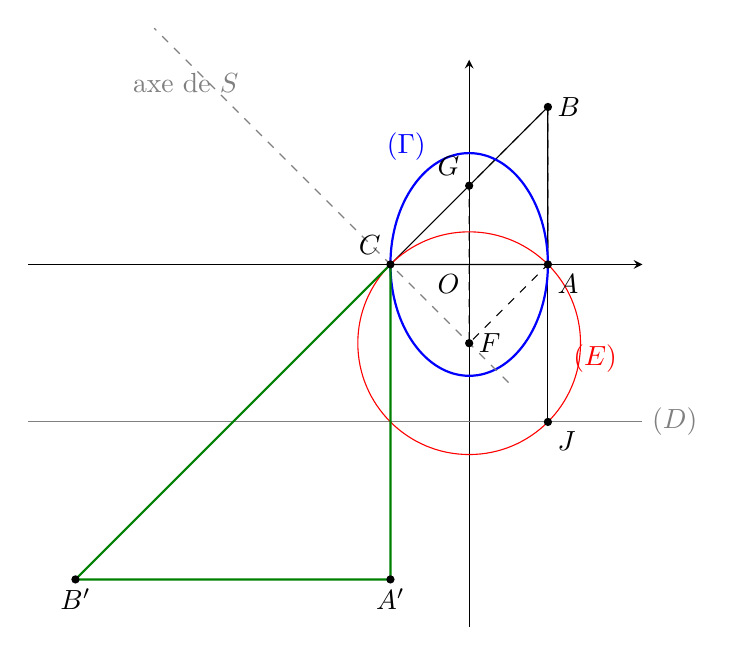
\begin{tikzpicture}[x=1cm,y=1cm,>=stealth]
	\draw[->] (-5.6,0) -- (2.2,0); \draw[->] (0,-4.6) -- (0,2.6);
	\draw[gray] (-5.6,-2) -- (2.2,-2) node[right] {$\D$};
	\draw (1,0) -- (1,2) -- (-1,0) -- cycle;
	\draw[thin] (1,2) -- (1,-2);
	\draw[dashed] (1,0) -- (1,2) -- (0,1) -- (0,-1) -- cycle;
	\draw[red] (0,-1) circle (1.4142);
	\draw[blue,thick] (0,0) ellipse (1 and 1.4142);
	\draw[green!50!black,thick] (-1,0) -- (-1,-4) -- (-5,-4) -- cycle;
	\draw[gray,dashed] (0.5,-1.5) -- (-4,3);
	\foreach \P/\L/\pos in {1/A/below right,-1/C/above left}
		\fill (\P,0) circle (1.5pt) node[\pos] {$\L$};
	\fill (1,2) circle (1.5pt) node[right] {$B$}; \fill (0,1) circle (1.5pt) node[above left] {$G$};
	\fill (0,-1) circle (1.5pt) node[right] {$F$}; \fill (1,-2) circle (1.5pt) node[below right] {$J$};
	\fill (-1,-4) circle (1.5pt) node[below] {$A'$}; \fill (-5,-4) circle (1.5pt) node[below] {$B'$};
	\node[below left] at (0,0) {$O$};
	\node[red] at (1.6,-1.2) {$(E)$}; \node[blue] at (-0.8,1.5) {$(\Gamma)$};
	\node[gray] at (-3.6,2.3) {axe de $S$};
\end{tikzpicture}
\end{center}
(Figure réduite : $1\cm$ pour une unité au lieu de $2\cm$.)
\begin{description}
	\item[Partie 1]
	\begin{enumerate}
		\item
		\begin{enumerate}
			\item \vln{Barycentre $F$ et parallélogramme $ABGF$ :}
				La somme des poids $2 - 1 + 1 = 2$ est non nulle et
				$\overrightarrow{AF} = \frac{-\overrightarrow{AB} + \overrightarrow{AC}}{2} = \frac{1}{2}\overrightarrow{BC} = \overrightarrow{BG}$.
				\par\noindent\ansbox{$F$ est le point tel que $\overrightarrow{AF} = \overrightarrow{BG}$ ($z_F = -i$).}
				L'égalité $\overrightarrow{AF} = \overrightarrow{BG}$ signifie que \par\noindent\ansbox{$ABGF$ est un parallélogramme.}
			\item \vln{Ensemble $(E)$ :}
				$2\overrightarrow{MA} - \overrightarrow{MB} + \overrightarrow{MC} = 2\overrightarrow{MF}$.
				La somme des poids de $2\overrightarrow{MA} - \overrightarrow{MB} - \overrightarrow{MC}$ est nulle : ce vecteur est constant,
				égal (avec $M = A$) à $-\overrightarrow{AB} - \overrightarrow{AC} = -2\overrightarrow{AG}$, de norme $2AG = BC = 2\sqrt{2}$.
				La condition s'écrit $2MF = 2\sqrt{2}$.
				\par\noindent\ansbox{$(E)$ est le cercle de centre $F$ et de rayon $\sqrt{2}$ (soit $2\sqrt{2}\cm$).}
				Il passe par $A$ et $C$ ($FA = FC = \sqrt{2}$).
		\end{enumerate}
		\item $z_J = 2z_A - z_B = 1 - 2i$ ; $\D$ est la droite d'équation $y = -2$ et, pour $M(x;y)$, $MH = |y + 2|$.
		\begin{enumerate}
			\item \vln{$A$ et $C$ sont sur $(\Gamma)$ :}
				Pour $M = A$ : $2 \times 0 - AB^2 + AC^2 = -4 + 4 = 0$ et $AH^2 - 4 = 2^2 - 4 = 0$.
				Pour $M = C$ : $2CA^2 - CB^2 + 0 = 8 - 8 = 0$ ($CB = 2\sqrt{2}$) et $CH^2 - 4 = 4 - 4 = 0$.
				\par\noindent\ansbox{$A \in (\Gamma)$ et $C \in (\Gamma)$.}
			\item \vln{Distances :}
				$FA = |1 + i|$, $FB = |1 + 3i|$, $FC = |-1 + i|$ :
				\par\noindent\ansbox{$FA^2 = 2$, $FB^2 = 10$, $FC^2 = 2$.}
			\item \vln{Nature de $(\Gamma)$ :}
				Relation de Leibniz : $2MA^2 - MB^2 + MC^2 = 2MF^2 + 2FA^2 - FB^2 + FC^2 = 2MF^2 + 4 - 10 + 2 = 2MF^2 - 4$.
				Donc (1) $\iff 2MF^2 - 4 = MH^2 - 4 \iff$ \par\noindent\ansbox{$2MF^2 = MH^2$.}
				Ainsi $\frac{MF}{MH} = \frac{1}{\sqrt{2}} = \frac{\sqrt{2}}{2}$ ; $F \notin \D$.
				\par\noindent\ansbox{$(\Gamma)$ est l'ellipse de foyer $F$, de directrice associée $\D$ et d'excentricité $\frac{\sqrt{2}}{2}$.}
				Avec $M(x;y)$ : $2\left(x^2 + (y+1)^2\right) = (y+2)^2 \iff 2x^2 + y^2 = 2 \iff x^2 + \frac{y^2}{2} = 1$ :
				ellipse de centre $O$, de demi-axes $1$ (sur $(Ox)$) et $\sqrt{2}$ (sur $(Oy)$), sommets $A$, $C$, $(0;\pm\sqrt{2})$.
		\end{enumerate}
	\end{enumerate}
	\item[Partie 2]
	\begin{enumerate}
		\item \vln{Affixes :}
			\ansbox{$z_C = -1$, $z_J = 1 - 2i$, $z_F = -i$.}
		\item
		\begin{enumerate}
			\item \vln{Expression complexe de $S$ :}
				$S : z' = a\bar{z} + b$ avec $a \neq 0$. $S(C) = C$ : $-a + b = -1$ ; $S(F) = J$ : $a \cdot i + b = 1 - 2i$.
				Par différence $a(1 + i) = 2 - 2i$, d'où $a = \frac{2 - 2i}{1 + i} = \frac{(2 - 2i)(1 - i)}{2} = -2i$, puis $b = -1 - 2i$.
				\par\noindent\ansbox{$S : z' = -2i\,\bar{z} - 1 - 2i$.}
			\item \vln{Éléments caractéristiques :}
				$|a| = 2$ : $S$ est une similitude indirecte de rapport $2$ ; son unique point invariant (rapport $\neq 1$) est $C$.
				On écrit $z' + 1 = -2i\left(\bar{z} + 1\right) = -2i\,\overline{(z + 1)}$ : $S = h \circ s$ où $h$ est l'homothétie de centre $C$ et de rapport $2$ et $s : z' + 1 = -i\,\overline{(z+1)}$ une réflexion d'axe passant par $C$.
				Les points invariants de $s$ vérifient, avec $w = z + 1$, $w = -i\bar{w}$ : $w = t(1 - i)$, $t \in \mathbb{R}$. L'axe est la droite passant par $C$ de vecteur directeur d'affixe $1 - i$, d'équation $y = -x - 1$.
				\par\noindent\ansbox{$S$ : similitude indirecte de centre $C$, de rapport $2$ et d'axe la droite $y = -x - 1$.}
		\end{enumerate}
		\item
		\begin{enumerate}
			\item \vln{Affixes de $A'$ et $B'$ :}
				$z_{A'} = -2i \times 1 - 1 - 2i$ et $z_{B'} = -2i(1 - 2i) - 1 - 2i = -2i - 4 - 1 - 2i$.
				\par\noindent\ansbox{$z_{A'} = -1 - 4i$ et $z_{B'} = -5 - 4i$.}
			\item \vln{Image du triangle $ABC$ :}
				C'est le triangle $A'B'C$ (car $S(C) = C$), rectangle isocèle en $A'$ avec $A'B' = A'C = 4$ (le double de $2$) et de sens indirect ; il est tracé sur la figure.
		\end{enumerate}
	\end{enumerate}
\end{description}
%%%%%%%%%%%%%%%%%%%%%%%%%%%%%%%%%%%%%%%%%%%%%%%%%%%%%%%%%%%%%%%%%%%%%%%%%%%%%%%%%%%%%%%%%%%%%%%%%%%%%%%%%%%%%%%%%%%%%%%%%%%%%%%%
\noindent \underline{\textsc{\textbf{PROBLEME II}}} (9 points)
\begin{description}
	\item[Partie A :]
	\begin{enumerate}
		\item
		\begin{enumerate}
			\item \vln{Continuité en $0$ :}
				$f(0) = 0 \cdot \expo{0} = 0$ ; $\lim_{x\to 0^-} x\expo{x} = 0$ ; $\lim_{x\to 0^+} \ln\left(2x + \sqrt{4x^2+1}\right) = \ln 1 = 0$.
				\par\noindent\ansbox{$f$ est continue en $0$.}
			\item \vln{Dérivabilité en $0$ :}
				À gauche : $\frac{f(x) - f(0)}{x} = \expo{x} \to 1$ ; à droite : $\frac{f(x)}{x} \to 2$ (admis).
				Les nombres dérivés à gauche ($1$) et à droite ($2$) sont différents.
				\par\noindent\ansbox{$f$ n'est pas dérivable en $0$ : point anguleux, demi-tangentes $y = x$ ($x \leq 0$) et $y = 2x$ ($x \geq 0$).}
		\end{enumerate}
		\item \vln{Variations de $f$ :}
			Pour $x < 0$ : $f'(x) = (1 + x)\expo{x}$, du signe de $1 + x$ ; $f(-1) = -\frac{1}{e}$ ; $\lim_{x\to-\infty} x\expo{x} = 0$.
			Pour $x > 0$ :
			\[ f'(x) = \frac{2 + \frac{4x}{\sqrt{4x^2+1}}}{2x + \sqrt{4x^2+1}} = \frac{2\left(\sqrt{4x^2+1} + 2x\right)}{\sqrt{4x^2+1}\left(2x + \sqrt{4x^2+1}\right)} = \frac{2}{\sqrt{4x^2+1}} > 0 ; \]
			$\lim_{x\to+\infty} f(x) = +\infty$.
			\[
			\begin{array}{c|ccccccc}
				x & -\infty & & -1 & & 0 & & +\infty \\ \hline
				f'(x) & & - & 0 & + & 1 \,\|\, 2 & + & \\ \hline
				 & 0 & & & & & & +\infty \\
				f & & \searrow & & \nearrow & 0 & \nearrow & \\
				 & & & -\frac{1}{e} & & & &
			\end{array}
			\]
		\item
		\begin{enumerate}
			\item \vln{Signe de $g'$ :}
				$g'(x) = 1 - \frac{2}{\sqrt{4x^2+1}}$. Pour $x \geq 2$, $\sqrt{4x^2 + 1} \geq \sqrt{17} > 2$, donc
				\par\noindent\ansbox{$g'(x) > 0$ sur $[2;+\infty[$.}
			\item \vln{Autre écriture de $f$ et limite de $g$ :}
				Pour $x > 0$ : $2x + \sqrt{4x^2+1} = 2x + x\sqrt{4 + \frac{1}{x^2}} = x\left(2 + \sqrt{4 + \frac{1}{x^2}}\right)$, d'où
				\par\noindent\ansbox{$f(x) = \ln x + \ln\left(2 + \sqrt{4 + \frac{1}{x^2}}\right)$.}
				Alors $g(x) = x - \ln x - \ln\left(2 + \sqrt{4 + \frac{1}{x^2}}\right) = x\left(1 - \frac{\ln x}{x}\right) - \ln\left(2 + \sqrt{4 + \frac{1}{x^2}}\right)$ ;
				$\frac{\ln x}{x} \to 0$ et le dernier logarithme tend vers $\ln 4$ :
				\par\noindent\ansbox{$\lim_{x\to+\infty} g(x) = +\infty$.}
			\item \vln{Tableau de $g$ et solution $\alpha$ :}
				$g(2) = 2 - \ln(4 + \sqrt{17}) \approx -0{,}09$ et $g(3) = 3 - \ln(6 + \sqrt{37}) \approx 0{,}51$.
				\[
				\begin{array}{c|ccc}
					x & 2 & & +\infty \\ \hline
					g'(x) & & + & \\ \hline
					 & & & +\infty \\
					g & & \nearrow & \\
					 & 2 - \ln(4+\sqrt{17}) & &
				\end{array}
				\]
				$g$ est continue, strictement croissante sur $[2;+\infty[$, et change de signe entre $2$ et $3$.
				\par\noindent\ansbox{$f(x) = x$ a une unique solution $\alpha$ dans $[2;+\infty[$, et $2 \leq \alpha \leq 3$ ($\alpha \approx 2{,}18$).}
				(Sur $\mathbb{R}$ tout entier, $0$ est aussi solution : l'unicité s'entend sur $[2;+\infty[$.)
		\end{enumerate}
		\item
		\begin{enumerate}
			\item \vln{$f(I) \subset I$ :}
				$f$ est croissante sur $I$ : $f(I) = [f(2) ; f(3)] = \left[\ln(4+\sqrt{17}) ; \ln(6 + \sqrt{37})\right] \approx [2{,}09 ; 2{,}49] \subset [2;3]$.
				\par\noindent\ansbox{Si $x \in I$, alors $f(x) \in I$.}
			\item \vln{Majoration de $f'$ :}
				Pour $x \in I$, $\sqrt{4x^2+1} \geq \sqrt{17} > 4$, donc $0 < f'(x) = \frac{2}{\sqrt{4x^2+1}} < \frac{2}{4} = \frac{1}{2}$.
				\par\noindent\ansbox{$0 \leq f'(x) \leq \frac{1}{2}$ sur $I$.}
				Par l'inégalité des accroissements finis entre $x$ et $\alpha$ (tous deux dans $I$), et comme $f(\alpha) = \alpha$ :
				\par\noindent\ansbox{$|f(x) - \alpha| \leq \frac{1}{2}|x - \alpha|$ pour tout $x \in I$.}
		\end{enumerate}
		\item
		\begin{enumerate}
			\item \vln{$u_n \in I$ :}
				$u_0 = 3 \in I$ ; si $u_n \in I$, alors $u_{n+1} = f(u_n) \in I$ (4.a). \par\noindent\ansbox{$u_n \in I$ pour tout $n$.}
			\item \vln{Inégalités :}
				Avec $x = u_n$ dans 4.(b) : \par\noindent\ansbox{$|u_{n+1} - \alpha| \leq \frac{1}{2}|u_n - \alpha|$.}
				Par récurrence, $|u_n - \alpha| \leq \left(\frac{1}{2}\right)^n|u_0 - \alpha|$ et $|u_0 - \alpha| = 3 - \alpha \leq 1$ :
				\par\noindent\ansbox{$|u_n - \alpha| \leq \left(\frac{1}{2}\right)^n$.}
			\item \vln{Rang $n_0$ :}
				$\left(\frac{1}{2}\right)^n \leq 0{,}1 \iff 2^n \geq 10 \iff n \geq 4$. On prend \par\noindent\ansbox{$n_0 = 4$.}
				$u_1 = f(3) \approx 2{,}4918$, $u_2 \approx 2{,}3092$, $u_3 \approx 2{,}2347$, \par\noindent\ansbox{$u_4 \approx 2{,}20$.}
				(On a en fait $\alpha \approx 2{,}177$.)
		\end{enumerate}
		\item
		\begin{enumerate}
			\item \vln{Branches infinies :}
				En $-\infty$ : $\lim f = 0$, \par\noindent\ansbox{l'axe des abscisses est asymptote horizontale en $-\infty$.}
				En $+\infty$ : $f(x) \to +\infty$ et
				\[ \frac{f(x)}{x} = \frac{\ln x}{x} + \frac{1}{x}\ln\left(2 + \sqrt{4 + \frac{1}{x^2}}\right) \to 0 . \]
				\par\noindent\ansbox{branche parabolique de direction $(Ox)$ en $+\infty$.}
			\item \vln{Tracé (figure réduite) :}
				Demi-tangentes en $O$ : $y = x$ à gauche, $y = 2x$ à droite. Valeurs : $f(-1) \approx -0{,}37$ ; $f(1) = \ln(2 + \sqrt{5}) \approx 1{,}44$ ; $f(5) \approx 2{,}30$ ; $f(10) \approx 3{,}69$.
				\begin{center}
				\begin{tikzpicture}[x=.8cm,y=.8cm,>=stealth]
					\draw[->] (-5.5,0) -- (10.5,0) node[below] {$x$};
					\draw[->] (0,-1.2) -- (0,4.5) node[left] {$y$};
					\foreach \t in {-5,-4,-3,-2,-1,1,2,3,4,5,6,7,8,9,10} \draw (\t,0.05) -- (\t,-0.05);
					\foreach \t in {-4,-2,2,4,6,8,10} \node[below] at (\t,-0.05) {\small $\t$};
					\foreach \t in {1,2,3,4} \draw (0.05,\t) -- (-0.05,\t) node[left] {\small $\t$};
					\draw[red] (-1,-1) -- (4.5,4.5) node[right] {$\D$};
					\draw[blue,thick] plot[domain=-5.5:0,samples=80] (\x,{\x*exp(\x)});
					\draw[blue,thick] plot[domain=0:10.5,samples=120] (\x,{ln(2*\x+sqrt(4*\x*\x+1))});
					\draw[gray,dashed] (-1,-1) -- (0,0) -- (1,2);
					\draw[dashed] (2.177,0) node[below] {\small $\alpha$} -- (2.177,2.177);
					\node[blue] at (8,3.1) {$\Courbe$};
				\end{tikzpicture}
				\end{center}
		\end{enumerate}
	\end{enumerate}
	\item[Partie B :]
	\begin{enumerate}
		\item \vln{Résolution de $(E_2)$ :}
			\ansbox{Les solutions de $y' - 2y = 0$ sont $x \mapsto C\expo{2x}$, $C \in \mathbb{R}$.}
		\item
		\begin{enumerate}
			\item \vln{Recherche de $u$ :}
				$u'(x) = (ax + a + b)\expo{x}$, donc $u'(x) - 2u(x) = (-ax + a - b)\expo{x}$.
				$u$ est solution de $(E_1)$ si et seulement si $-ax + a - b = x$ pour tout $x$, soit $-a = 1$ et $a - b = 0$.
				\par\noindent\ansbox{$a = b = -1$ : $u(x) = -(x+1)\expo{x}$.}
			\item \vln{Équivalence :}
				$(\varphi + u)' - 2(\varphi + u) = (\varphi' - 2\varphi) + (u' - 2u) = (\varphi' - 2\varphi) + x\expo{x}$.
				\par\noindent\ansbox{$\varphi + u$ est solution de $(E_1)$ $\iff$ $\varphi' - 2\varphi = 0$, c'est-à-dire $\varphi$ solution de $(E_2)$.}
			\item \vln{Solutions de $(E_1)$ :}
				\ansbox{$y(x) = C\expo{2x} - (x+1)\expo{x}$, $C \in \mathbb{R}$.}
		\end{enumerate}
		\item \vln{Solution nulle en $0$ :}
			$y(0) = C - 1 = 0 \iff C = 1$. \par\noindent\ansbox{$y(x) = \expo{2x} - (x+1)\expo{x}$.}
	\end{enumerate}
\end{description}
